\documentclass{report}

\usepackage[italian]{babel} % Imposta la lingua italiana
\usepackage{tcolorbox}
\usepackage{forest}
\usepackage{dirtree} % Aggiungi il pacchetto dirtree
\usepackage{graphicx} % Aggiungi il pacchetto graphicx
\usepackage{pgfplots}
\usepackage{wrapfig}
\usepackage{amsmath}
\usepackage{circuitikz}
\pgfplotsset{width=5cm,compat=1.9}

\renewcommand{\thefootnote}{\roman{footnote}}
% Definizione del nuovo ambiente 'important'
\newtcolorbox{important}[1][]{
  colback=yellow!10!white,
  colframe=red!50!black,
  title=Ricorda,
  #1
}
% Definizione del nuovo ambiente 'definition'
\newtcolorbox{definition}[1][]{
  colback=blue!10!white,
  colframe=blue!50!black,
  title=Definizione,
  #1
}

\begin{document}

\begin{center}
  \vspace*{2cm}
  {\Huge Fisica sperimentale I \par}
  \vspace{1cm}
  
\includegraphics[width=0.5\textwidth]{logounibs.png}\par
  \vspace{1cm}
  {\Large Riccardo Rasori \par}
  \vspace{0.5cm}
  {\large A.A. 2024/2025 \par}
  \vspace{2cm}
\end{center}

\tableofcontents % Aggiungi l'indice

\chapter{Introduzione}

\section{Il metodo scientifico}
La natura è complessa $\rightarrow$ per capirla si fanno esperimenti\\
Es. Tolta l'aria (nel vuoto) tutti i corpi cadono in maniera uguale
\\
$\rightarrow$ Gli esperimenti formulano una teoria\\
$\rightarrow$ La fisica usa il linguaggio matematico per le teorie e le leggi\\
\section{Grandezze fisiche}
\begin{definition}
  \textbf{Misurazione}: si associa un numero (misura) a una grandezza fisica. Associa anche la sua attendibilità (errore).\\
  Deve essere non ambigua e riproducibile.
\end{definition}
\begin{definition}
  \textbf{Grandezza fisica}: è definita in relazione al procedimento/strumento utilizzato per misurare.\\
  Non tutte le grandezze sono indipendenti (velocità $\frac{m}{s}$).
\end{definition}
\dirtree{%
  .1 Sistema Internazionale.
  .2 Tempo (s).
  .2 Lunghezza (m).
  .2 Massa (kg).
  .2 Quantità di materia (mol).
  .2 Temperatura (K).
  .2 Intensità di corrente elettrica (A).
  .2 Intensità luminosa (cd).
}
\subsection{Tempo}
Grandezza fisica misurata con l'orologio.\\
Si usa l'orologio atomico basato sulla frequenza di una transizione iperfine all'atomo di $^{133}Cs$ (Cesio)
\begin{definition}
  \textbf{Secondo}: tempo che ci mette la luce emessa da $^{133}Cs$ per fare $9.192.631.770$ vibrazioni.
\end{definition}
\subsection{Lunghezza}
Si usa il regolo per misurarla
\begin{definition}
  \textbf{Metro}: distanza percorsa dalla luce nel vuoto in $\frac{1}{299.792.458}$ di secondo.
\end{definition}
\subsection{Massa}
\begin{definition}
  \textbf{Massa}: grandezza fisica misurata con bilancia a due bracci.
\end{definition}
Campione di riferimento: kg $\rightarrow$ cilindro di platino-iridio per definire la massa
\section{La notazione scientifica}
\dirtree{%
.1 Vantaggi.
.2 È formalmente compatta.
.2 È evidente l'\underline{ordine di grandezza} $\rightarrow$ {Potenza di 10 con cui è espresso il numero}.
.2 È evidente la precisione con cui è noto il valore numerico $\rightarrow$ L'incertezza è espressa dal suo errore\\ {Es. $l=(3,5\pm0,1)m$}.
}
L'errore ci dice quante cifre significative usare per rappresentare una grandezza\\
Es. $(4,5397\pm0,21)*10^{3} \leftarrow$ se già la prima cifra è incerta per l'errore, non ha senso precisare tutto quello che c'è dopo (397)
\\
$\rightarrow$ va scritto $(4,54\pm0,21)*10^{3}$
\subsection{Num cifre significative}
3m $\rightarrow$ per l'errore può essere $3\pm0,1$ m (2, 3 o 4)\\
3,0m $\rightarrow$ per l'errore può essere $3,0\pm0,1$ m (2,9; 3,0; 3,1)\\
0,003m $\leftarrow$ 1 cifra significativa\\
0,0030m $\leftarrow$ 2 cifre significative\\

\subsubsection{Addizione}
\begin{center}

  \begin{tabular}{r}
    18,0      \\
    + 0,0039  \\
    + 0,00002 \\
    \hline
    18,00392  \\
    = 18,0
  \end{tabular}

\end{center}\footnote{deve contenere un numero di cifre significative uguale a quello del numero con incertezza maggiore}

\subsubsection{Moltiplicazione}
Il risultato \underline{di norma} deve contenere tante cifre significative quante ne sono contenute nel fattore con meno cifre significative
\begin{center}

  \begin{tabular}{r}
    Es:     \\
    2,21    \\
    $* 0,3$ \\
    \hline
    0,663   \\
    = 0,7
  \end{tabular}
\end{center}
Es. $12,4*84=1041,6=1,04*10^{3}$
\subsubsection{Divisione}
Vale la stessa regola della moltiplicazione\\
Es. $14,28/0,714=20=20,0$ oppure $2,0*10^{1}$\\
Es. $0,032/0,004=8=0,8*10^{1}$\\
Es: $9,83/9,3$\footnote{2 cifre, ma l'incertezza è circa dell'1\%}$=1,05698924731=1,06$\footnote{Se avessi scritto 1,1 l'incertezza era circa del 10\%, quindi metto 1,06 e l'incertezza rimane circa 1\%}\\
\section{Meccanica}
\begin{itemize}
  \item \textbf{Cinematica}: studio del moto indipendente dalle cause
  \item \textbf{Dinamica}: studio del moto in relazione alle forze agenti
  \item \textbf{Statica}: studio del moto in assenza di forze
\end{itemize}
\subsection{Cinematica}
\begin{itemize}
  \item Si studia un corpo puntiforme (particella) in cui è incentrata la massa
  \item Lo studiamo in modo unidimensionale (si muove solo in una direzione) (moto rettilineo)
        \begin{itemize}
          \item Posizione
          \item Spostamento
          \item Velocità
          \item Accelerazione
        \end{itemize}
  \item In natura esistono corpi puntiformi (elettroni)
        \begin{itemize}
          \item Hanno raggio $<2*10^{-20}$ m
        \end{itemize}
\end{itemize}
\subsubsection{Moto}
\begin{itemize}
  \item Il suo concetto è relativo
        \begin{itemize}
          \item Per un osservatore un oggetto potrebbe essere in movimento, per un altro potrebbe essere fermo
        \end{itemize}
  \item \underline{Sistema di riferimento}
        \begin{itemize}
          \item Definisce la posizione di un corpo
          \item Assi x y z
          \item In cinematica il sistema di rif. è arbitrario (1,2,3 dimensioni)
          \item La \underline{posizione} p la coordinata lungo l'asse della particella
          \item Lo \underline{spostamento} è la differenza tra il valore della pos. finale e quella iniziale\\$\Delta x=x_2-x_1$
          \item Conviene descrivere il moto con il variare della posizione in funzione del tempo\\Ho la funzione $x(t)$ dove il tempo è la variabile indipendente\\\begin{tikzpicture}
                  \begin{axis}[
                      axis x line=middle,
                      axis y line=middle,
                      enlargelimits,
                      xtick={1,2,3,4},
                      xlabel={$t$},
                      ylabel={},
                      ytick=\empty,
                      samples=100,
                      grid=major
                    ]
                    % Disegna la curva interpolata
                    \addplot[smooth, tension=0.8, thick, blue] coordinates {
                        (0,-2) (2,-1) (3,1) (4,2)
                      };

                    % Disegna i punti con cerchi vuoti
                    \addplot[only marks, mark=o, mark size=3pt] coordinates {
                        (0,-2) (2,-1) (3,1) (4,2)
                      };
                  \end{axis}
                \end{tikzpicture}
          \item La velocità è quanto rapidamente si muove la particella
                \begin{itemize}
                  \item Velocità vettoriale media\\È il rapporto tra lo spostamento $\Delta x$ che si verifica in un certo intervallo $\Delta t$ e l'intervallo stesso\\$\overline{v}=\frac{\Delta x}{\Delta t}=\frac{x_2(t_2)-x_1(t_1)}{t_2-t_1}[\frac{m}{s}]$\\$[\overline{v}]=[LT^{-1}]$\\\begin{tikzpicture}
                          \begin{axis}[
                              axis x line=middle,
                              axis y line=middle,
                              enlargelimits,
                              xtick={1,2,3,4},
                              xlabel={$t$},
                              ylabel={},
                              ytick=\empty,
                              samples=100,
                              grid=major
                            ]

                            % Disegna la curva interpolata
                            \addplot[smooth, tension=0.8, thick, blue] coordinates {
                                (1,-4) (3,0)  (4,2)
                              };

                            % Disegna i punti con cerchi vuoti
                            \addplot[only marks, mark=o, mark size=3pt] coordinates {
                                (1,-4) (3,0)  (4,2)
                              };

                            % Disegna la retta secante (velocità media tra due punti)
                            \addplot[domain=0.5:4.5, thick, green] {1.5*x - 4};

                          \end{axis}
                        \end{tikzpicture}
                        \\
                        Può succedere che la particella si muova e che torni nello stesso punto:
                        \begin{itemize}
                          \item lo spostamento è 0 $\Rightarrow$ la velocità vettoriale media è 0
                        \end{itemize}
                  \item Velocità scalare media\\$\overline{u}=\frac{l}{\Delta t}[m/s]$\\$[\overline{u}]=[LT^{-1}]$
                  \item Velocità istantanea\\
                        \begin{definition}
                          Limite della velocità vettoriale media quando $\Delta t$ tende a 0
                        \end{definition}$v(t)=\lim_{\Delta t\to0}\frac{\Delta x}{\Delta t}=\lim_{t \to t_1}\frac{x(t)-x(t_1)}{t-t_1}=\lim_{\Delta t\to0}\frac{x(t+\Delta t)-x(t)}{\Delta t}\Rightarrow v(t)=\frac{dx(t)}{dt}\rightarrow$ è la derivata prima di x(t) rispetto al tempo t\\
                        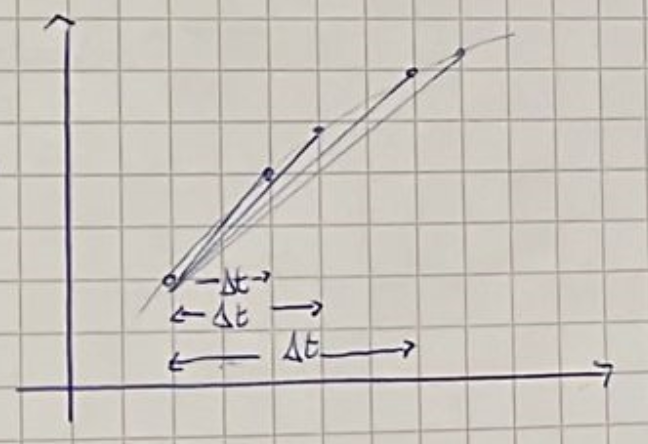
\includegraphics[scale=0.5]{grafico3.png}
                \end{itemize}
          \item Esempi di moti
                \begin{itemize}
                  \item Particella con velocità costante\\$x(t)=A+Bt$\\Velocità istantanea\\$v(t)=\frac{dx}{dt}=\frac{d}{dt}(A+Bt)=0+B$
                  \item Particella accelerata uniformemente
                \end{itemize}
          \item Accelerazione media o istantanea
                \begin{itemize}
                  \item Media: rapporto tra la variazione della velocità della particella in un $\Delta t$ e l'intervallo stesso\\$\overline{a}=\frac{\Delta v}{\Delta t}=\frac{v_2(t_2)-v_1(t_1)}{t_2-t_1}$\\$[\overline{a}]=[\frac{LT^{-1}}{T}]=[LT^{-2}]\rightarrow[\frac{m}{s^2}]$
                  \item Istantanea:\\$a(t)=\lim_{\Delta t\to0}\frac{\Delta v}{\Delta t}=\lim_{t\to t_1}\frac{v(t)-v(t_1)}{t-t_1}=\lim_{\Delta t\to0}\frac{v(t+\Delta t)-v(t)}{\Delta t}=\frac{dv(t)}{dt}=\frac{d^2xt}{dt^2}\rightarrow $ è la derivata seconda di x(t) rispetto al tempo t
                  \item Accelerazione e velocità concordi
                        \begin{itemize}
                          \item Parlo di accelerazione se la velocità aumenta
                          \item Parlo di decelerazione se la velocità diminuisce
                        \end{itemize}
                        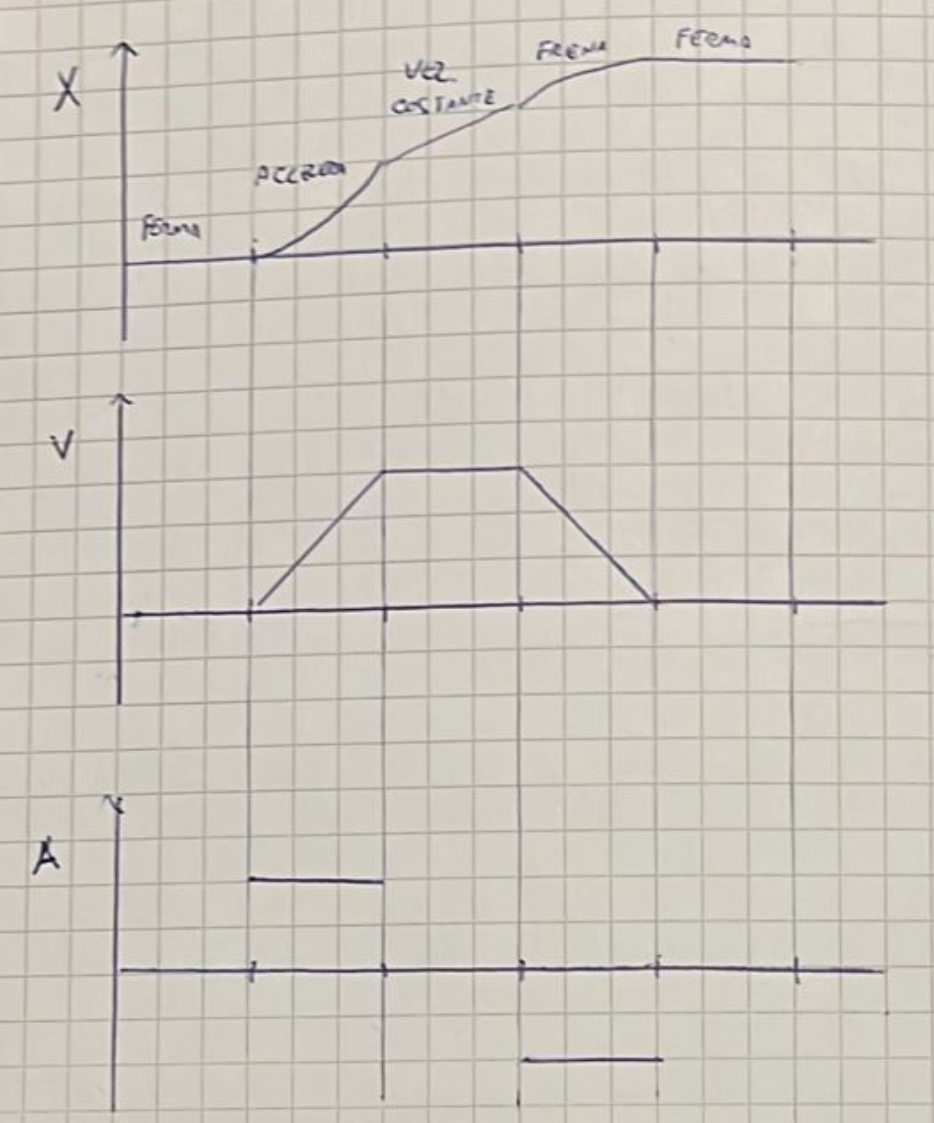
\includegraphics[scale=0.5]{grafico4.png}
                \end{itemize}
          \item Accelerazione costante
                \begin{itemize}
                  \item Trovo la velocità\\a(t)=costante e poniamo per semplicità $t_0=0$\\$a=\overline{a}=\frac{\delta v}{\delta t}=\frac{v-v_0}{t-0}\Rightarrow v(t)=v_0+a*t (1)$
                        \begin{center}
                          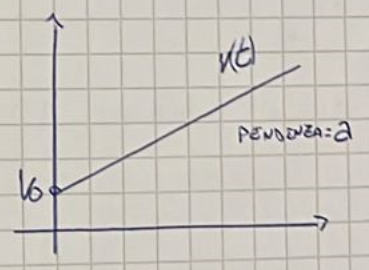
\includegraphics[scale=0.5]{grafico5.png}
                        \end{center}
                  \item Trovo la posizione\\
                        \begin{equation}
                          \begin{cases}
                            \overline{v}=\frac{1}{2}(v_0+v)=\frac{1}{2}(v_0+v_0+a*t)=v_0+\frac{1}{2}a*t \\
                            \overline{v}=\frac{\delta x}{\delta t}=\frac{x-x_0}{t-0}
                          \end{cases}
                        \end{equation}
                        $\Rightarrow x(t)=x_0+v_0*t+\frac{1}{2}a*t^2$ (2)\\
                        Posso conoscere dove si trova la particella a patto di sapere le condizioni iniziali di tempo e moto della particella\begin{center}
                          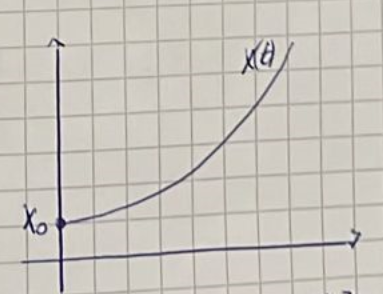
\includegraphics[scale=0.5]{grafico6.png}
                        \end{center}
                \end{itemize}
                Posso ricavare altre equazioni
                \begin{itemize}
                  \item eliminando t da (1) e (2)\\$v^2(x)=v_0^2+2a(x-x_0) (3)$
                  \item eliminando a da (1) e (2)\\$x(t)=x_0+\frac{v_0+v}{2}t (4)$
                  \item eliminando $v_0$ da (1) e (2)\\$x(t)=x_0+v(t)-\frac{1}{2}a(t^2) (5)$
                \end{itemize}
                La (1) e la (2) sono le più importanti, da sapere a memoria\\
                Mostriamo come a questi risultati si può arrivare anche con le derivate\\
                $a=\frac{dv}{dt}\Rightarrow dv=a*dt\Rightarrow \int_{x_0}^{x}dx=\int_{0}^{t}vdt=\int_{0}^{t}(v_0+a*t)dt \Rightarrow x-x_0=v_0*t+\frac{1}{2}a*t^2 \Rightarrow x=x_0+v_0*t+\frac{1}{2}a*t^2$\\
                Se al posto di $t_0$ avesso un t qualunque uso $t-t_0$\\
        \end{itemize}
  \item Moto di caduta libera\\In assenza della resistenza dell'aria tutti i corpi cadono ugualmente
        \begin{itemize}


          \item $g=9,81\frac{m}{s^2}$
          \item La direzione (detta vericale) è la stessa direzione dell'accelerazione di gravitò\\Sostituendo alle equazioni precedenti $a=-gt$ $x_0=0$ \\$v=v_0+at=-gt$\\$x=x_0+v_0t+\frac{1}{2}at=-\frac{1}{2}gt^2$
        \end{itemize}
\end{itemize}
\chapter{Vettori}
Le grandezze fisiche sono:
\begin{itemize}
  \item \textbf{Scalari:} definite da un numero e un'unità di misura
  \item \textbf{Vettoriali:} è definita da un numero, una direzione e un verso\\Il prodotto delle grandezze vettoriali è lo \underline{spostamento}
\end{itemize}
\section{Spostamento}
Lo spostamento da A a B è caratterizzato dalla sua intensità, dalla direzione e dal verso e si indica con
\begin{center}
  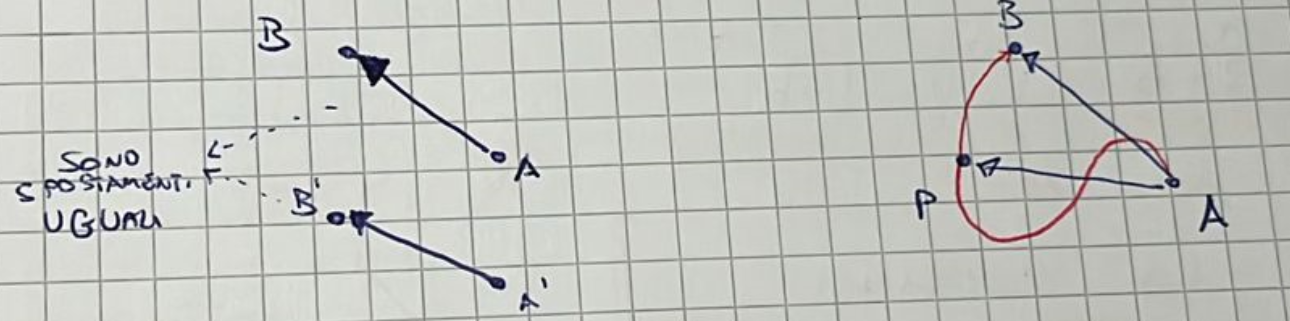
\includegraphics[scale=0.3]{img1.png}

\end{center}
\begin{itemize}
  \item Tutte le grandezze fisiche che si comportano come lo spostamento sono vettori\\Notazioni vettoriali\\\begin{tabular}{cc}
          \textbf{Vettore} & \textbf{Modulo} \\
          {AB}             & $\overline{AB}$ \\
          v                & v               \\
          $\vec{V}$        & $|\vec{V}|$
        \end{tabular}
\end{itemize}
\section{Somma di vettori: Metodo grafico}

$\vec{A}+\vec{B}=\vec{s}$\\
\underline{non} è la somma dei moduli\\
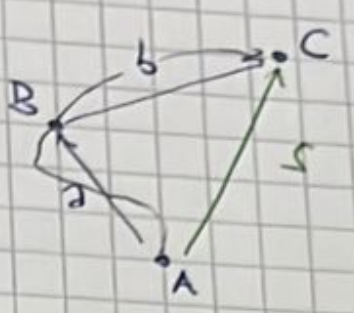
\includegraphics[scale=0.3]{img2.png}

Proprietà della somma
\begin{itemize}
  \item Commutativa: $\vec{a}+\vec{b}=\vec{b}+\vec{a}$
  \item Associativa: $(\vec{a}+\vec{b})+\vec{c}=\vec{a}+(\vec{b}+\vec{c})$\\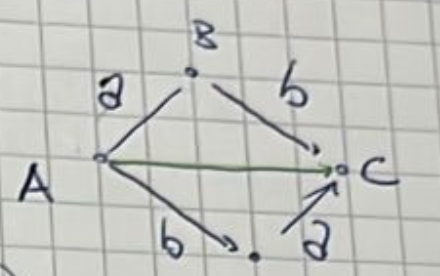
\includegraphics[scale=0.3]{img3.png}
\end{itemize}
\section{Sottrazione}
Il vettore $-\vec{b}$ ha la stessa intensità di $\vec{b}$, ma verso opposto\\
La differenza è la somma di $\vec{a}$ e $-\vec{b}$\\
$\vec{a}-\vec{b}=\vec{a}+(-\vec{b})$\\
\section{Componenti dei vettori}
Proietto le componenti sull'asse delle x\\
$a_x=a\cos\theta$\\
$a_y=a\sin\theta$\\
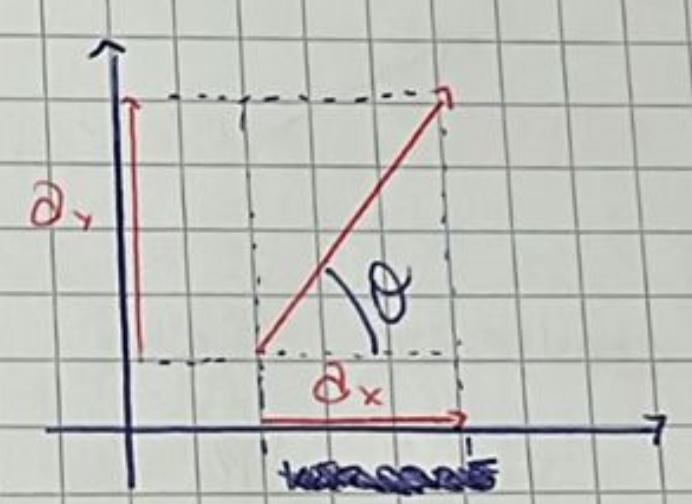
\includegraphics[scale=0.3]{img4.png}
Le componenti:
\begin{itemize}
  \item Sono scalari
  \item Insieme definiscono in modo univoco il vettore\\$|a|=\sqrt{a_x^2+a_y^2}$\\$\tan\theta=\frac{a_y}{a_x}$
\end{itemize}
\section{Versori}
\begin{definition}
  Un \textbf{versore} è un vettore con modulo=1
\end{definition}
\begin{figure}[!ht]

  \resizebox{0.5\textwidth}{!}{%
    \begin{circuitikz}
      \tikzstyle{every node}=[font=\LARGE]
      \draw [->, >=Stealth] (8,10.75) -- (13.25,10.75);
      \draw [->, >=Stealth] (8,10.75) -- (8,15.25);
      \draw [->, >=Stealth] (8,10.75) -- (5,8.25);
      \draw [ color={rgb,255:red,255; green,0; blue,0}, ->, >=Stealth] (8,10.75) -- (6.5,9.5);
      \draw [ color={rgb,255:red,255; green,0; blue,0}, ->, >=Stealth] (8,10.75) -- (9.75,10.75);
      \draw [ color={rgb,255:red,255; green,0; blue,0}, ->, >=Stealth] (8,10.75) -- (8,12.5);
      \node [font=\LARGE, color={rgb,255:red,255; green,0; blue,0}] at (8.5,11.75) {k};
      \node [font=\LARGE, color={rgb,255:red,255; green,0; blue,0}] at (8.75,10.25) {j};
      \node [font=\LARGE, color={rgb,255:red,255; green,0; blue,0}] at (7,10.75) {i};
    \end{circuitikz}
  }%
  \label{fig:my_label}
\end{figure}
i, j, k sono i versori della terna cartesiana destrorsa\\
Si indicano anche con $\hat{i}, \hat{j}, \hat{k}$\\


\end{document}